% ~~~~~~~~~~~~~~~~~~~~~~~~~~~~~~~~~~~~~~~~
%% INTRODUCTION
% ~~~~~~~~~~~~~~~~~~~~~~~~~~~~~~~~~~~~~~~~
\chapter{Introduction}
The Simulation Experiment Description Markup Language (SED-ML) is an XML-based format for describing simulation experiments, including model changes, calibrations, simulations, analyses, and computations and visualizations of simulation results.

The number of computational models of biological systems is growing at an ever increasing pace.
At the same time, their size and complexity are also increasing. It is now generally accepted that one must be able to exchange the mathematical structure of such models, for instance to build on existing studies by reusing models or to reproduce model results. The efforts to standardize the representation of computational models in various areas of biology, such as the Systems Biology Markup Language (SBML) \citep{Hucka:2003}, CellML \citep{cuellar:2003} or NeuroML \citep{Goddard:2001}, resulted in an increase of the exchange and re-use of models. However, the description of models is not sufficient to reproduce, reuse, and combine simulation experiments and their results. One also needs to describe the procedures the models are subjected to, i.e., the information required to reproduce simulation experiments among users and software tools. The increasing use of computational simulation experiments to inform modern biological research creates new challenges to reproduce, annotate, archive, and share such experiments.

SED-ML is a computer-readable exchange format for describing simulation experiments. Critically, SED-ML can be used with a wide range of model formats, modeling frameworks, simulation algorithms, and simulation tools. For many simulation experiments, SED-ML can capture the information in the Minimum Information About a Simulation Experiment (MIASE) \citep{Waltemath:2011} guidelines.

SED-ML is developed as a community project and defined via this technical specification and a corresponding XML Schema. 

This document describes \currentLV of SED-ML, which is the successor of \previousLV (published in \citep{smith2021sedl1v4} and originally described in \citep{WAB+11}).

%-----------------------------------------------------------------------------
\subsection{Color conventions in this document}
\label{sec:notation}
%-----------------------------------------------------------------------------

Throughout this document, we use coloring to carry additional
information for the benefit of those viewing the document on media
that can display color:

\begin{itemize}

\item We use a \changed{red color} in text and a \textcolor[rgb]{0.0117, 0.0664, 0.5742}{dark blue color} in figures to indicate changes
  between this version of the specification, namely SED-ML Level~1 Version~4, and
  the \emph{most recent previous release} of the specification
  (which, for the present case, is SED-ML Level~1 Version~3).  The changes may be either
  additions or deletions of text; in the case of deletions, entire
  sentences, paragraphs or sections are colored to indicate a
  change has occurred inside them.  In UML diagrams, blue text and/or lines are used to indicate semantic changes or additions.

\item We use a \textcolor{blue}{blue color} in text to indicate a hyperlink from one
  point in this document to another.  When viewed in electronic form, clicking
  on blue-colored text will cause a jump to the
  section, figure, table or page to which the link refers.

\end{itemize}




% ~~~~~~~~~~~~~~~~~~~~~~~~~~~~~~~~~~~~~~~~
%% OVERVIEW
% ~~~~~~~~~~~~~~~~~~~~~~~~~~~~~~~~~~~~~~~~
\section{SED-ML overview}
SED-ML specifies for a given simulation experiment

\begin{itemize}
\item which datasets to use (\hyperref[class:dataDescription]{DataDescription});
\item which models to use (\Model);
\item which modifications to apply to models before simulation or other analyses (\hyperref[class:change]{Change});
\item which simulation, model calibration, or other analysis procedures to run on each model (\Simulation and \AbstractTask);
\item how to post-process the results of these simulations and analysis (\DataGenerator); and
\item how these results should be presented and exported as figures and tables (\hyperref[class:output]{Output}).
\end{itemize}

A \hyperref[class:sed-ml]{SED-ML document} contains the following main objects to describe this information: \hyperref[class:dataDescription]{DataDescription}, \Model, \Simulation, \AbstractTask, \DataGenerator, and \Output.

\paragraph*{\hyperref[class:dataDescription]{DataDescription}}
The \hyperref[class:dataDescription]{DataDescription} class enables investigators to specify datasets for a simulation experiment. Such data can be used for instance to parameterize model simulations or to plot data together with simulation results.

\paragraph*{\Model}
The \Model class enables investigators to describe the externally-defined models involved in a simulation experiment.

\paragraph*{\Simulation}
The \Simulation class enables investigators to describe the settings required for each simulation and analysis. These includes information such as the type of each simulation/analysis, the algorithm required to execute the simulation/analysis, and the algorithm parameters that the simulation/analysis should be executed with.

\paragraph*{\AbstractTask}
The \AbstractTask's three child classes (\Task, \RepeatedTask, and \ParameterEstimationTask) enable investigators to specify an execution of an experiment through a combination of a \Simulation or \FitExperiment with a \Model. This allows investigators to describe a variety of different experiment formats in a flexible way.

\paragraph*{\DataGenerator}
The \DataGenerator class enables investigators to encode post-processing of simulation/analysis results before the generation of outputs, e.g., one can normalize the result of an observable, or calculate the mean of several observables. In the definition of a \DataGenerator, any addressable variable or parameter of any model or \DataSource may be referenced, and used to calculate new values using \hyperref[sec:mathML]{MathML}.

\paragraph*{\Output}
The \hyperref[class:output]{Output} class enables investigators to describe how post-processing simulation results should be exported, such as with two dimensional plots (\hyperref[class:plot2D]{Plot2D}), three dimensional plots (\hyperref[class:plot3D]{Plot3D}), and data tables (\hyperref[class:report]{Report}).

Detailed technical information about these classes is available in Chapter~\ref{chp:specification}. 

% ~~~~~~~~~~~~~~~~~~~~~~~~~~~~~~~~~~~~~~~~
%% EXAMPLE SIMULATION
% ~~~~~~~~~~~~~~~~~~~~~~~~~~~~~~~~~~~~~~~~
\section{Example simulation experiment}
\label{motivation:example}
This section illustrates an example simulation experiment for the repressilator model \citep{Elowitz:2000}. The corresponding SED-ML is listed in Appendix~\ref{example:repressilator}. A \hyperref[sec:archive]{COMBINE archive} for this simulation experiment is available as \texttt{L1V3\char`_repressilator.omex} at \url{https://sed-ml.org/}.

Additional example SED-ML files are available in Appendix~\ref{app:examples}. Numerous complete examples with model files are available as COMBINE archives at \url{https://sed-ml.org/}.

The repressilator is a synthetic oscillating network of transcription regulators in \textit{Escherichia coli}. The network is composed of the three repressor genes Lactose Operon Repressor (\code{lacI}), Tetracycline Repressor (\code{tetR}) and Repressor CI (\code{cI}), which code for proteins binding to the promoter of the other, blocking their transcription. The three inhibitions form a cyclic negative-feedback loop. To describe the interactions of the molecular species involved in the network, the authors built a simple mathematical model of coupled first-order differential equations. All six molecular species included in the network (three mRNAs, three repressor proteins) participate in creation (transcription/translation) and degradation processes. The model was used to determine the influence of the various parameters on the dynamic behavior of the system. In particular, parameter values were sought which induce stable oscillations in the concentrations of the system components.

%% ~~ TIME-COURSE ~~
\subsection{Time-course simulation}
\label{sec:timecourse}
Figure~1c of the reference publication \citep{Elowitz:2000} (reproduced with SED-ML in \fig{rep_tc1} and \fig{rep_tc2}) reported the following simulation. 

\begin{itemize}
 	\item{\changed{The \Model imports the repressilator model} identified by the Unified Resource Identifier (URI) \citep{Berners-Lee:2005}\\ \url{https://www.ebi.ac.uk/biomodels/model/download/BIOMD0000000012?filename=BIOMD0000000012_url.xml}.}
 	\item{\changed{The \Simulation defines a uniform time course simulation for 1000 minutes, recording output each minute, using CVODE (KISAO:0000019).}}
        \item{\changed{Several \DataGenerator elements and an \Output are used to define a 2D plot of \code{lacI}, \code{tetR} and \code{cI} against time.}}
 \end{itemize}

\begin{figure}[ht]
    \centering
    \begin{minipage}{0.47\textwidth}
        \centering
        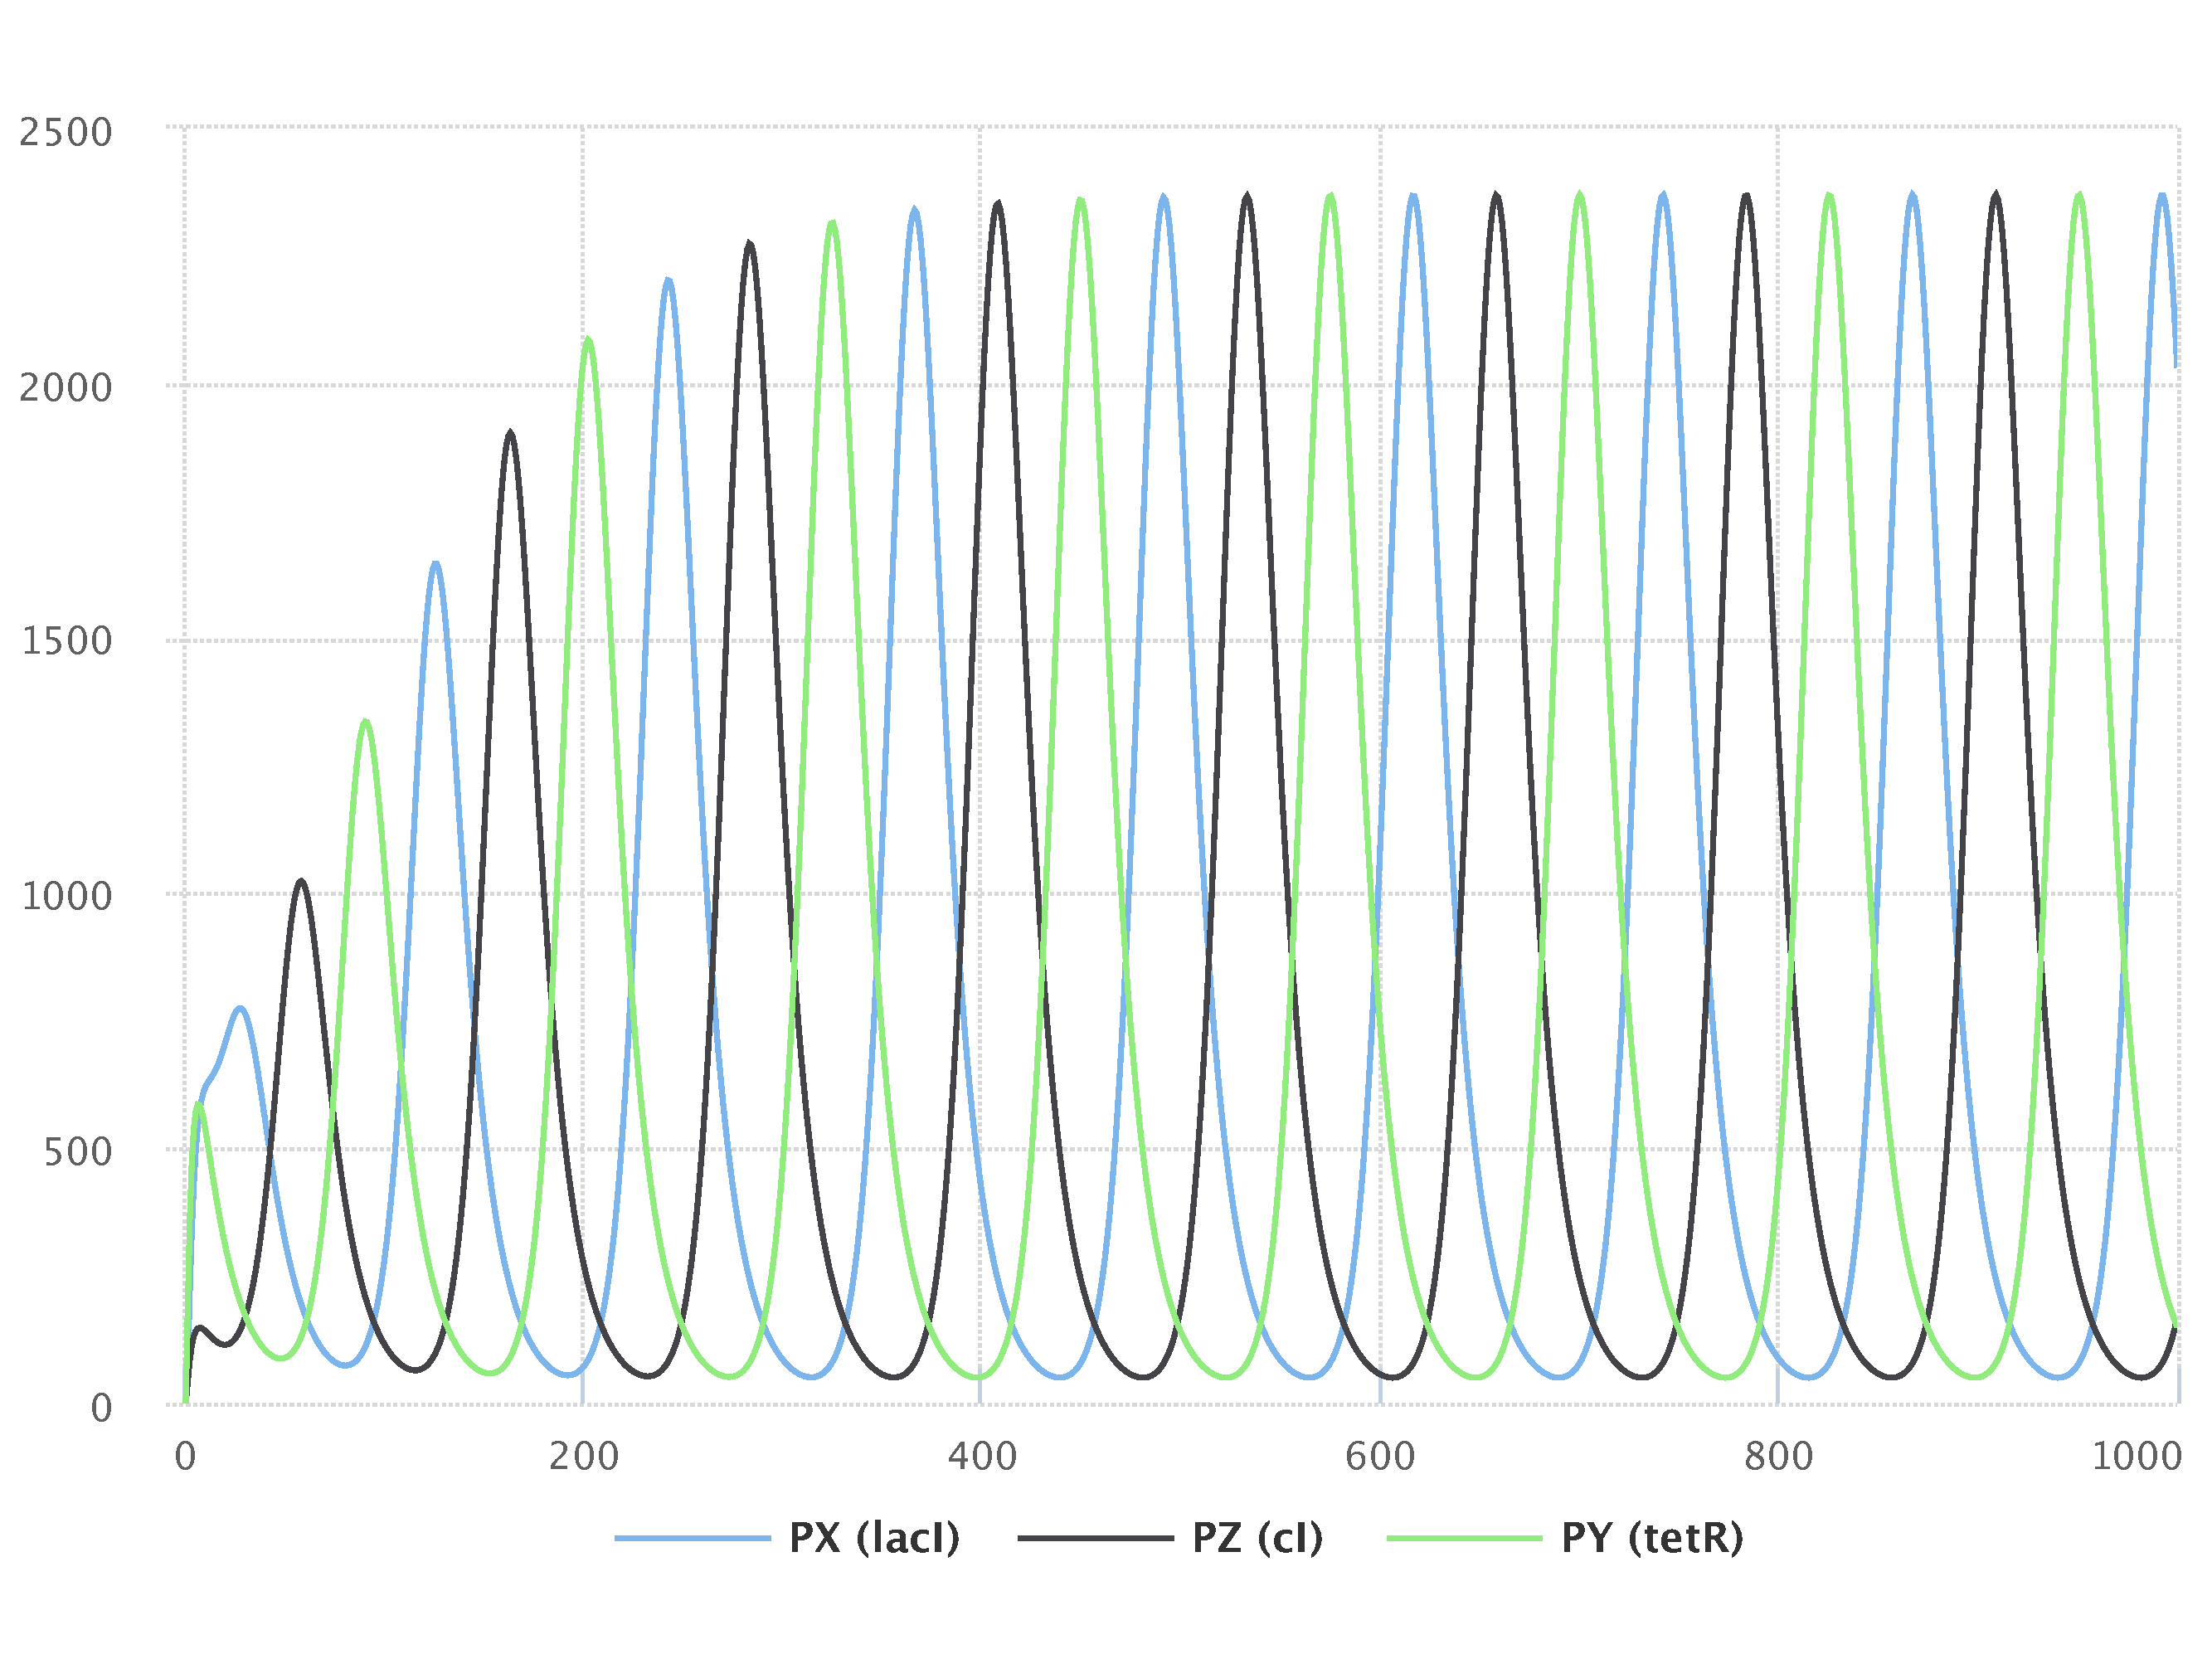
\includegraphics[width=1.0\textwidth]{examples/repressilator/results/sedml_webtools/timecourse}
        \caption{Time-course simulation of the repressilator depicting repressor proteins lacI, tetR and cI. Simulation with SED-ML web tools \citep{bergmann2017sed}.}
        \label{fig:rep_tc1}
    \end{minipage}\hfill
    \begin{minipage}{0.47\textwidth}
        \centering
        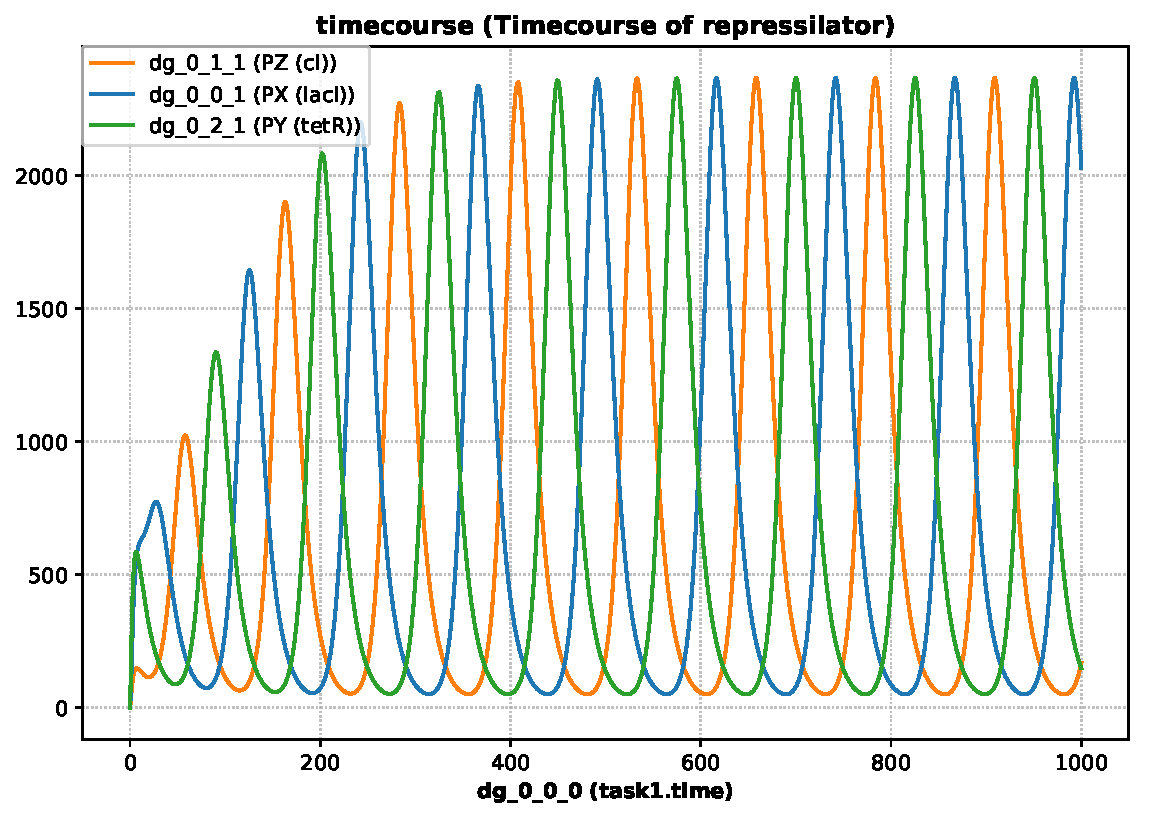
\includegraphics[width=1.0\textwidth]{examples/repressilator/results/tellurium/timecourse}
        \caption{Time-course simulation of the repressilator depicting repressor proteins lacI, tetR and cI. Simulation with tellurium \citep{tellurium}.}
        \label{fig:rep_tc2}
    \end{minipage}
\end{figure}


%% ~~ PRE-PROCESSING ~~
\subsection{Applying pre-processing}
\label{sec:preprocessing}
A common step in a simulation experiment is the modification of model parameters before simulation. When changing the parameter values for the protein copies per promoter, \code{tps$\_$repr}, and the leakiness in protein copies per promoter, \code{tps$\_$active}, as illustrated below, the system's behavior switches from sustained oscillations to damped oscillations (\fig{rep_pre1} and \fig{rep_pre2}).

\begin{itemize}
	\item{\changed{Everything is defined as in Section~\ref{sec:timecourse} above.}}
	\item{\changed{Two child \Change elements of the \Model are defined that change the value of the parameter \code{tps$\_$repr} from \code{0.0005} to \code{1.3e-05}, and \code{tps$\_$active} from \code{0.5} to \code{0.013}.}}
	\item{\changed{The same \Simulation, \DataGenerator, and \Output elements are used.}}
\end{itemize}

\pagebreak

\begin{figure}[ht]
    \centering
    \begin{minipage}{0.47\textwidth}
        \centering
        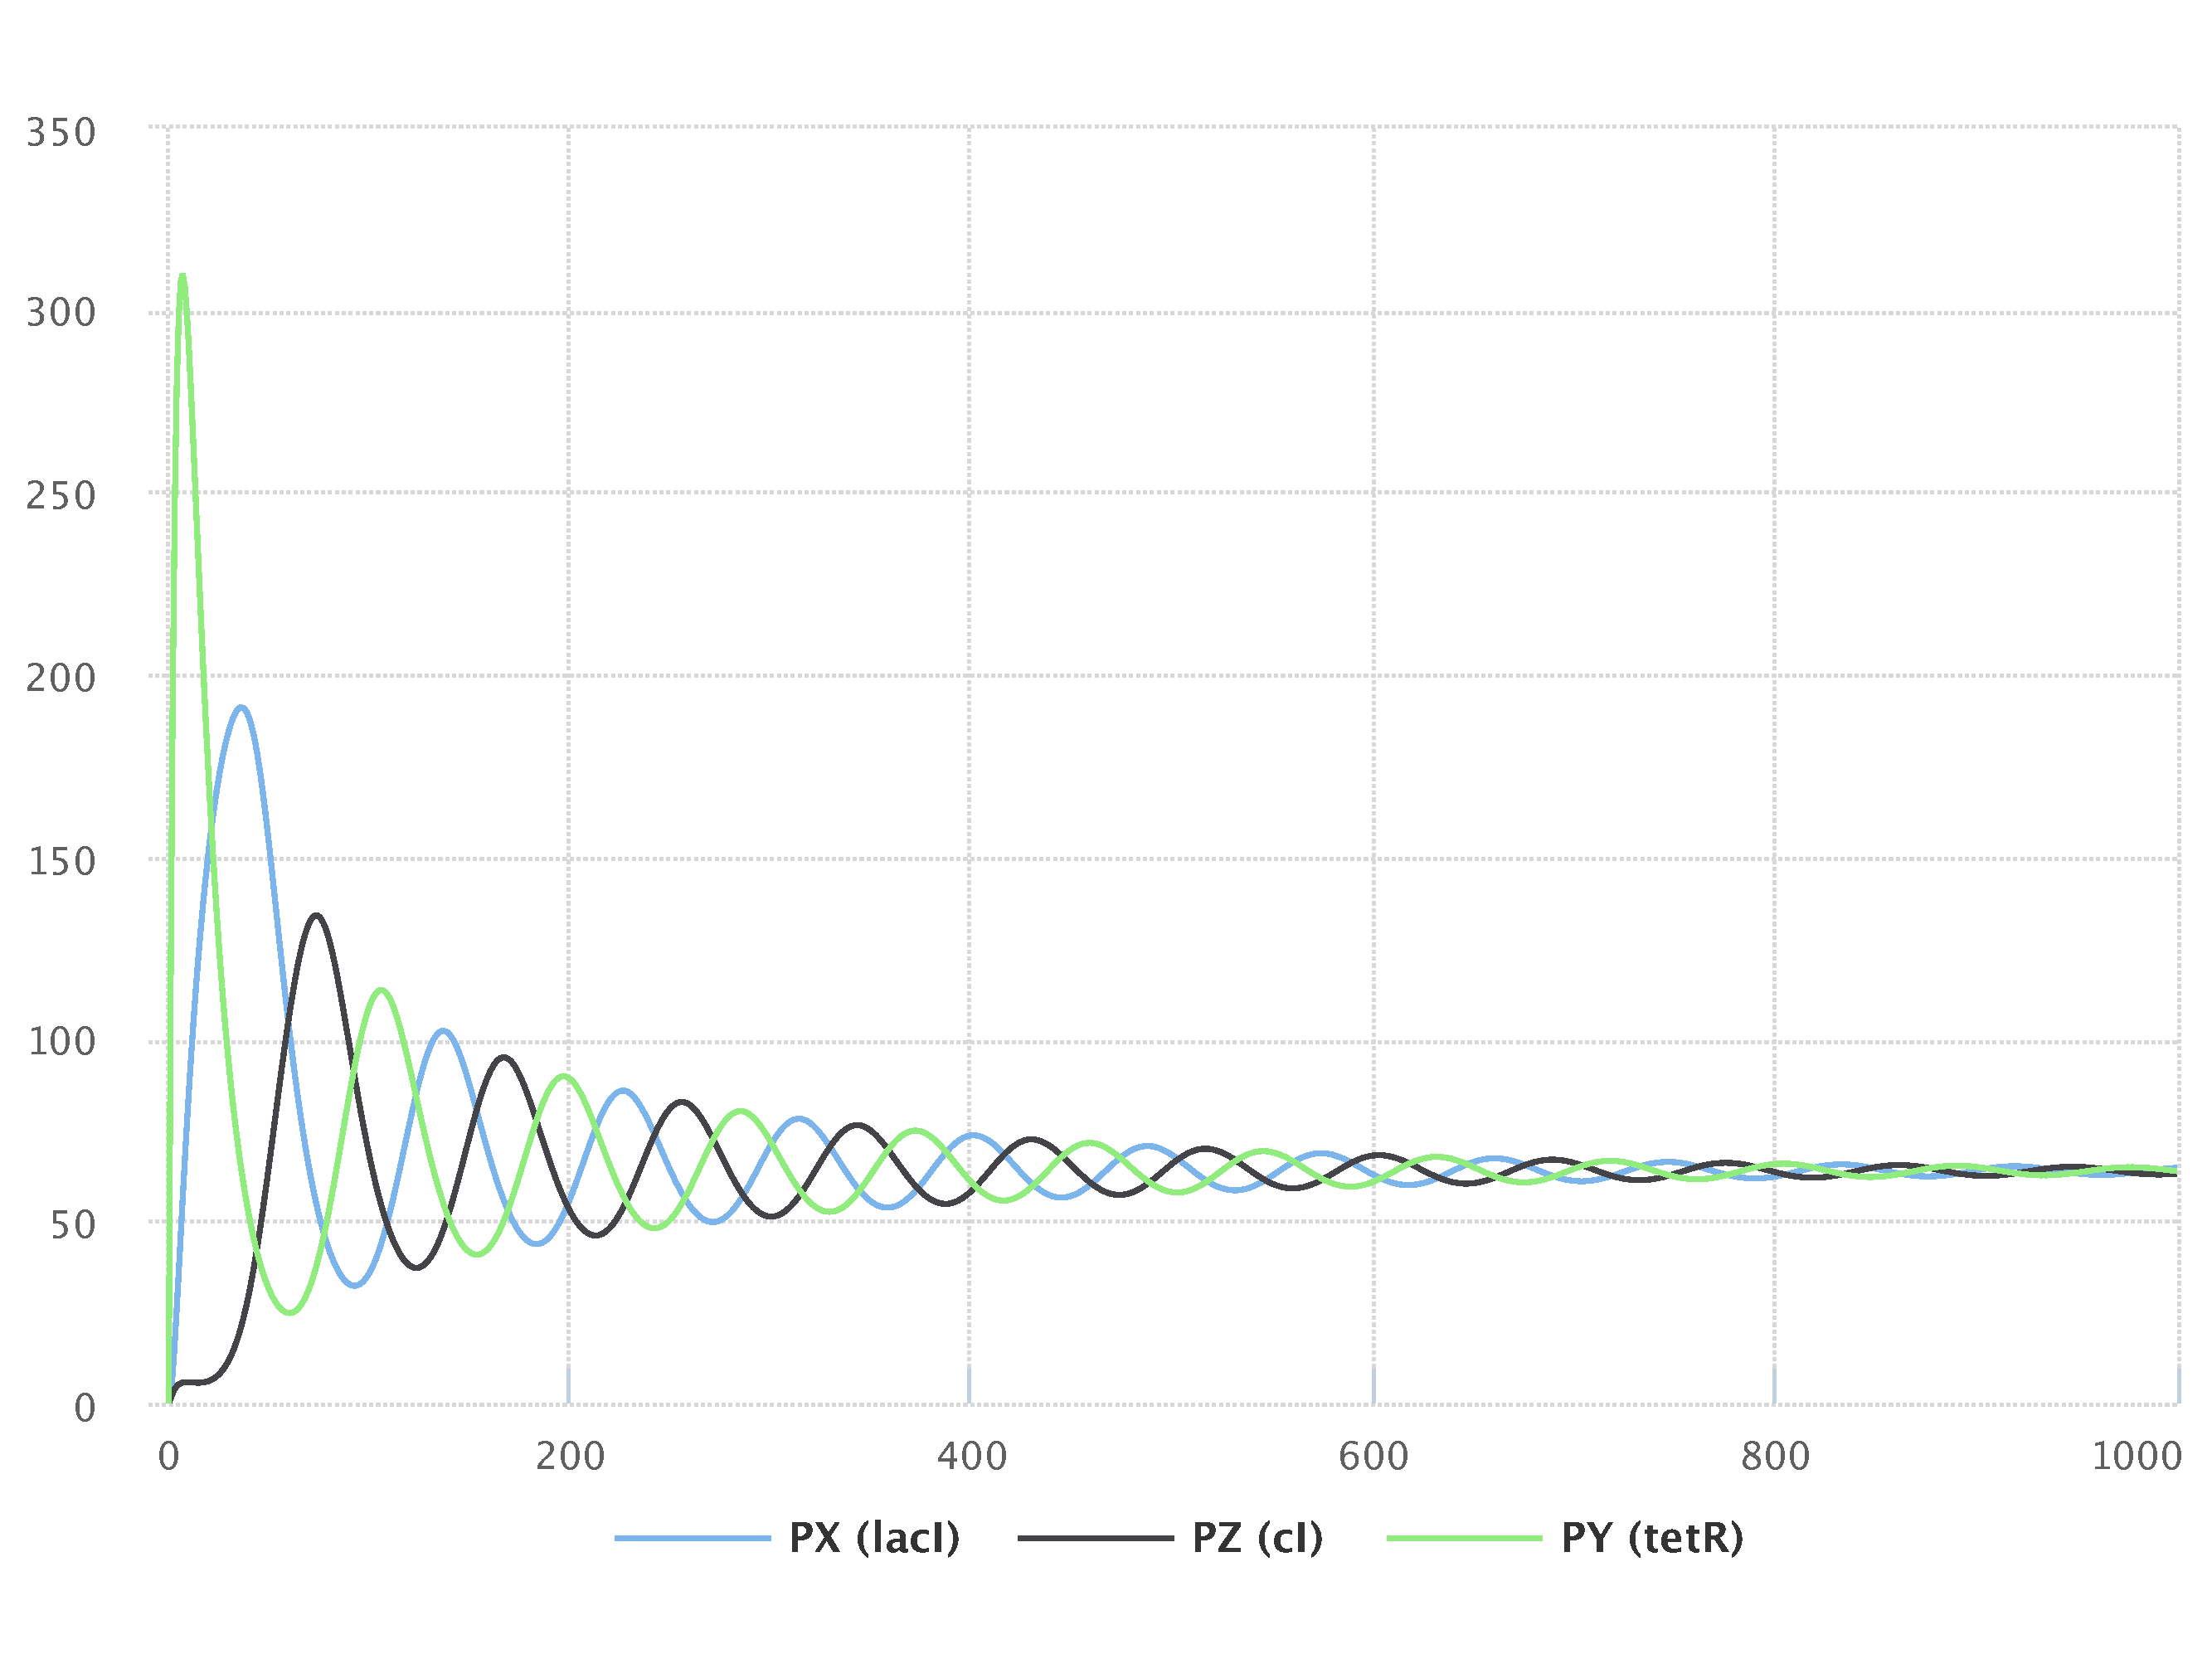
\includegraphics[width=1.0\textwidth]{examples/repressilator/results/sedml_webtools/preprocessing}
        \caption{Time-course simulation of the repressilator after changing parameters \code{tps$\_$repr} and \code{tps$\_$active}. Simulation with SED-ML web tools \citep{bergmann2017sed}.}
        \label{fig:rep_pre1}
    \end{minipage}\hfill
    \begin{minipage}{0.47\textwidth}
        \centering
        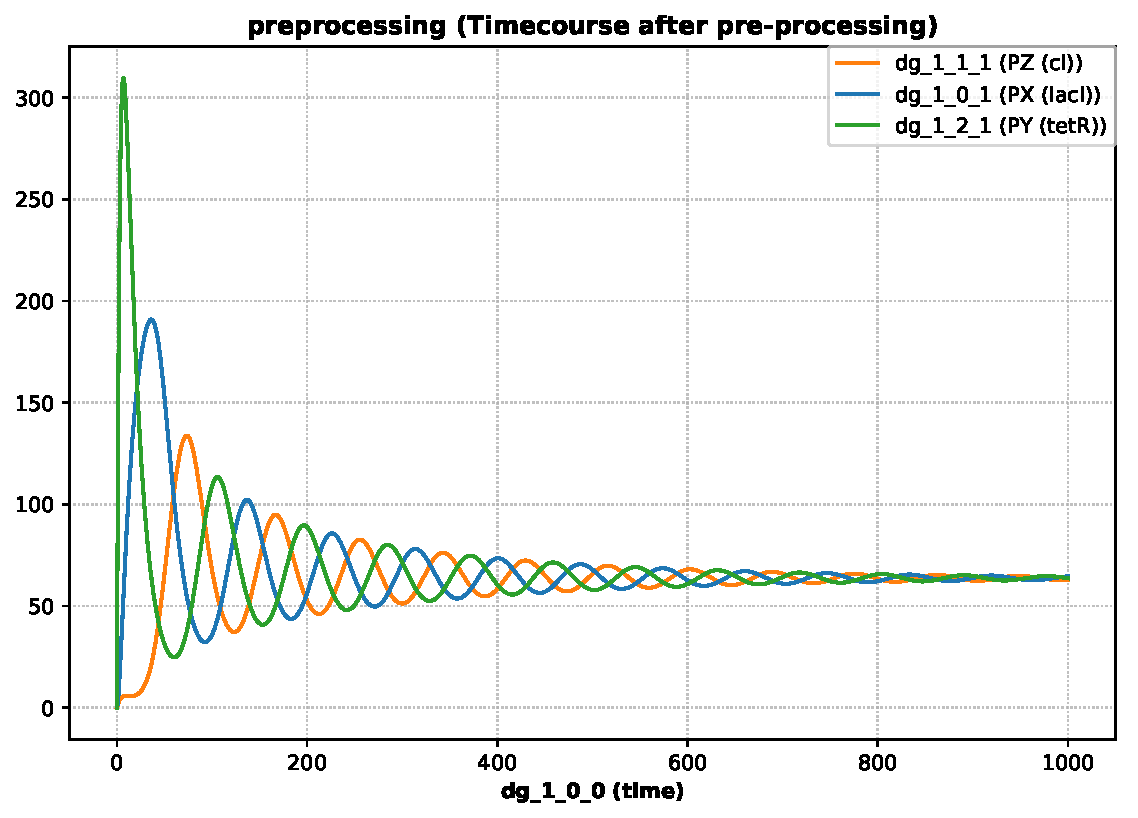
\includegraphics[width=1.0\textwidth]{examples/repressilator/results/tellurium/preprocessing}
        \caption{Time-course simulation of the repressilator after changing parameters \code{tps$\_$repr} and \code{tps$\_$active}. Simulation with tellurium \citep{tellurium}.}
        \label{fig:rep_pre2}
    \end{minipage}
\end{figure}


%% ~~ POST-PROCESSING ~~
\subsection{Applying post-processing}
\label{sec:postprocessing}
In a simulation experiment, the raw numerical output of simulations must often be post-processed before plotting or reporting. Normalized plots (\fig{rep_post1} and \fig{rep_post2}) of the results of the first simulation (Section~\ref{sec:timecourse}), which highlights the influence of the variables on each other (in phase-plane), can be constructed as follows:

\begin{itemize}
	\item{\changed{Everything is initially defined as in Section~\ref{sec:timecourse} above.}}
        \item{\changed{Three new \DataGenerator elements are defined that normalize the values of \code{lacI(t)}, \code{tetR(t)} and \code{cI(t)} by dividing each by their respective maximums.}}
	\item{\changed{A new 2D plot \Output is created where these normalized values are plotted against each other:  \code{lacI} vs. \code{cI}, \code{cI} vs. \code{tetR}, and \code{tetR} vs. \code{lacI}.}}
\end{itemize}

\begin{figure}[ht]
    \centering
    \begin{minipage}{0.47\textwidth}
        \centering
        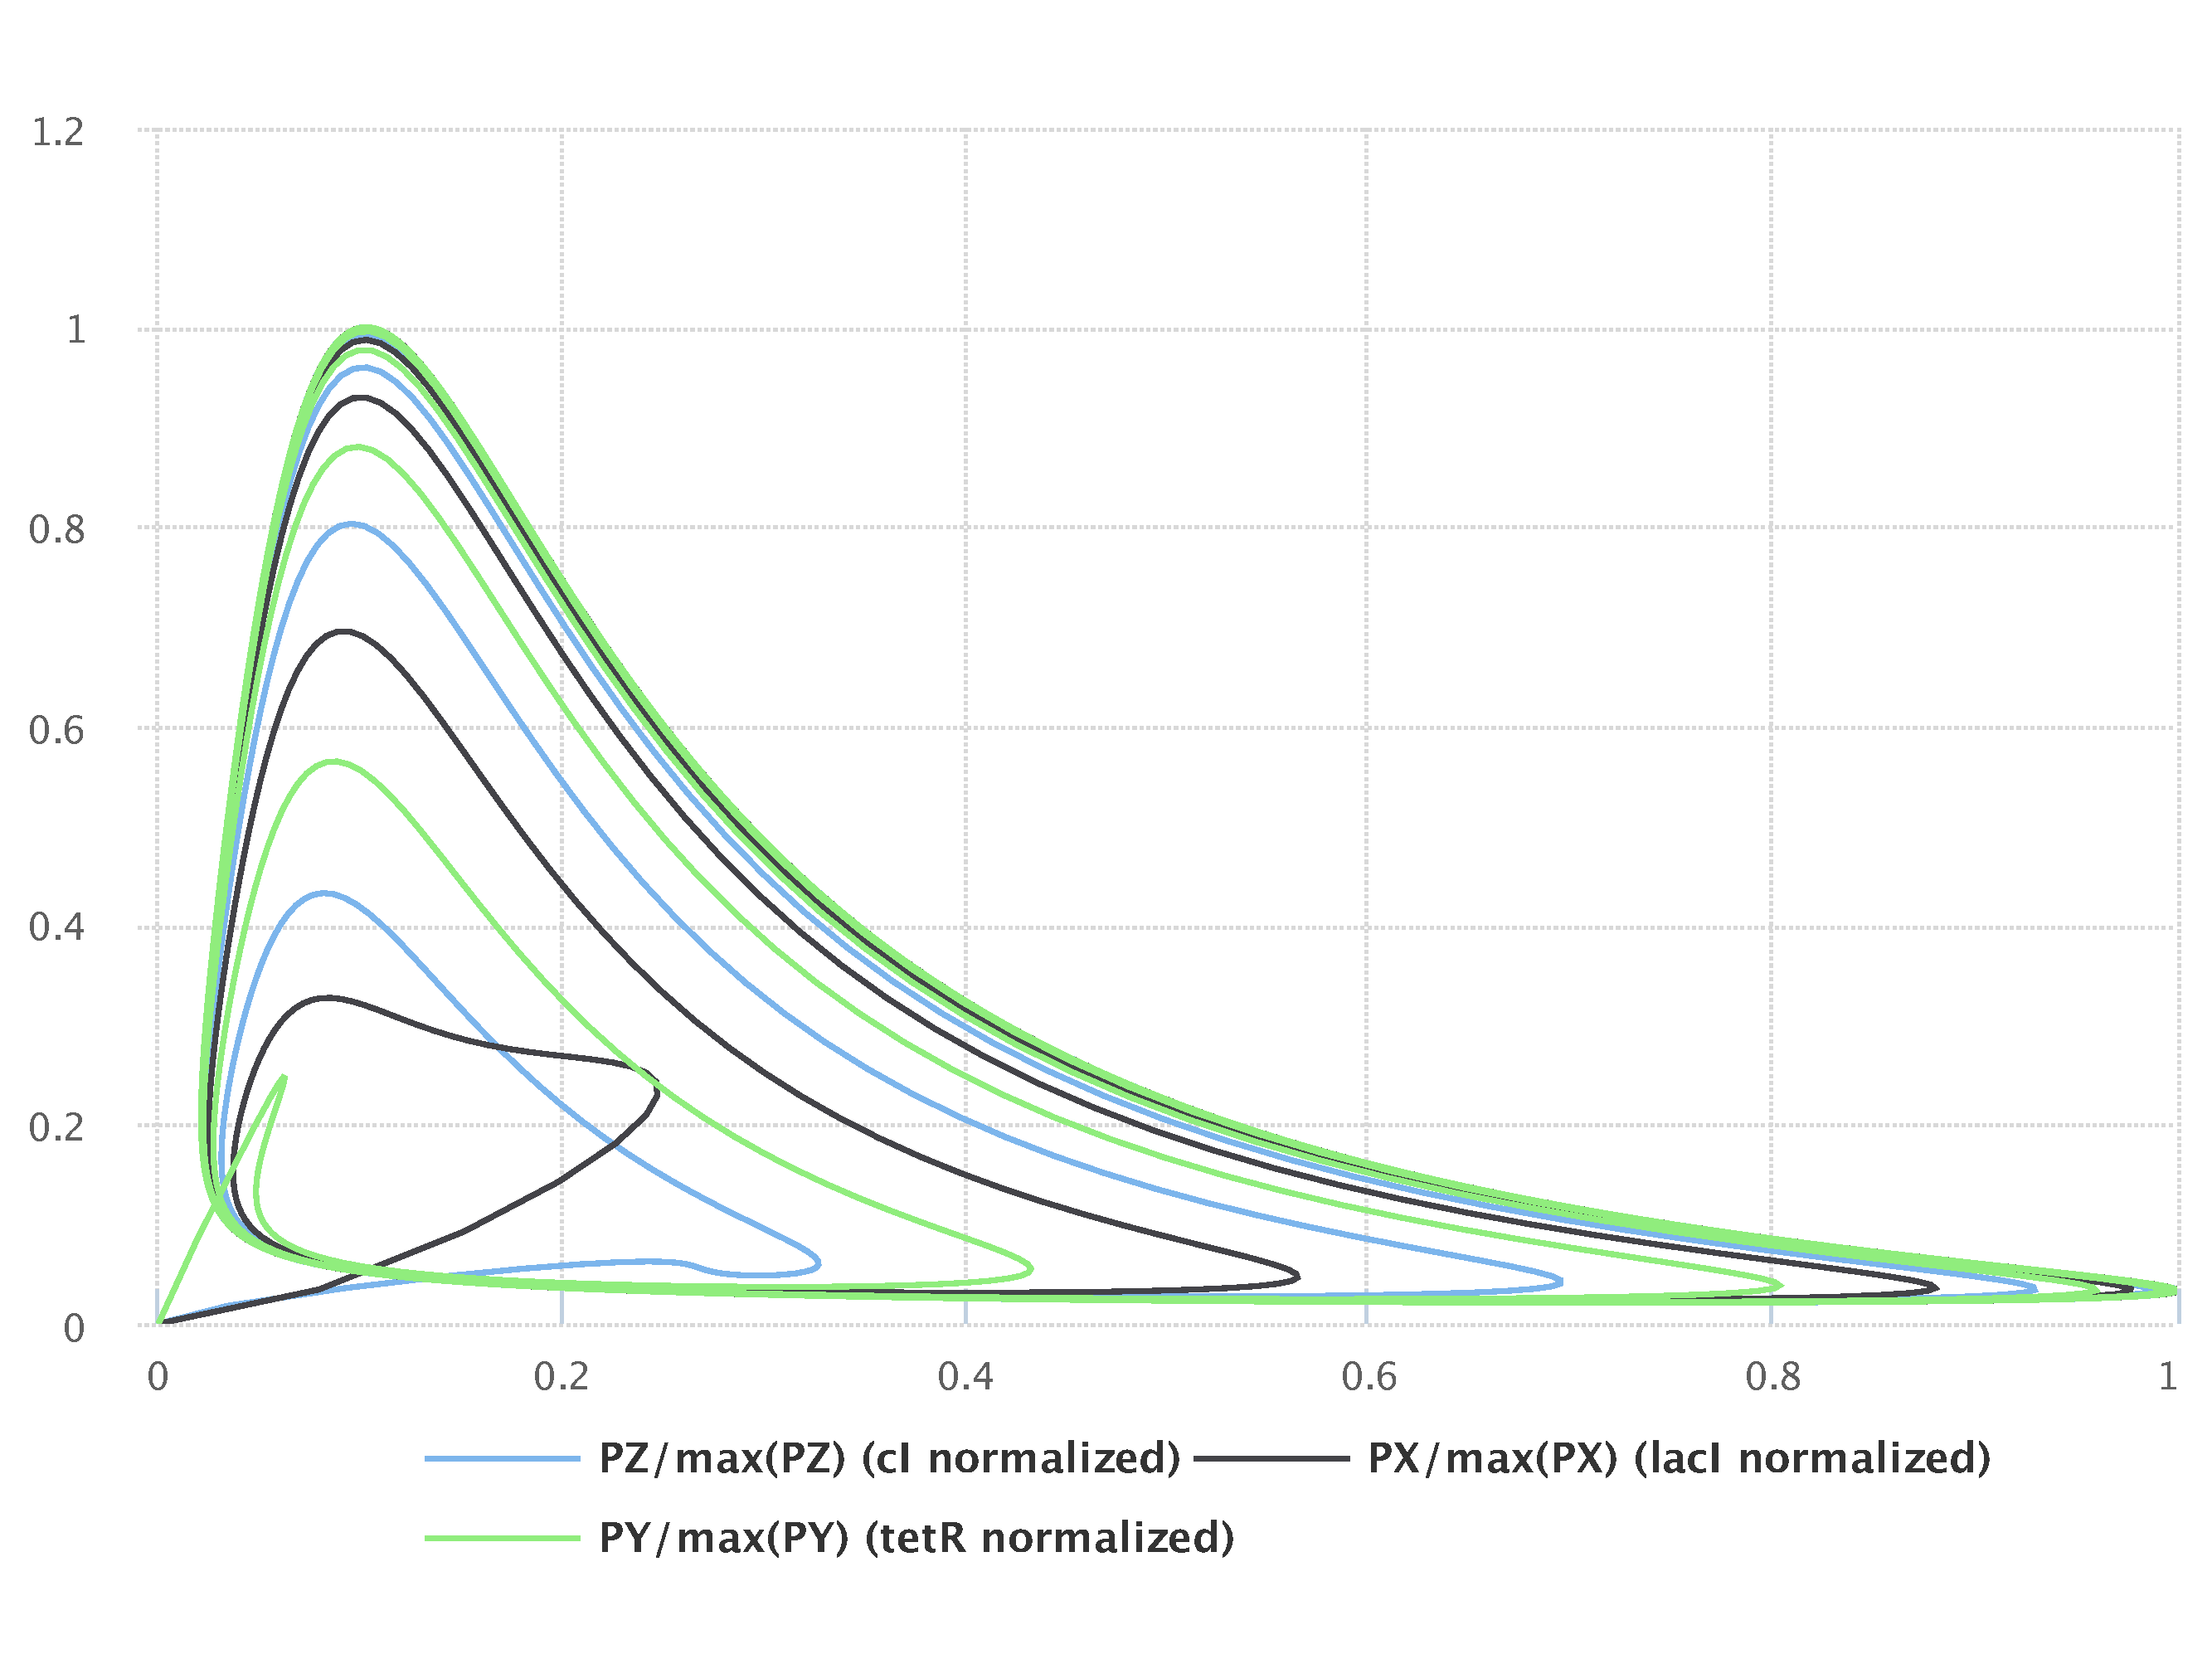
\includegraphics[width=1.0\textwidth]{examples/repressilator/results/sedml_webtools/postprocessing}
        \caption{Time-course simulation of the repressilator. Normalized \code{lacI}, \code{tetR} and \code{cI} in phase-plane. Simulation with SED-ML web tools \citep{bergmann2017sed}.}
        \label{fig:rep_post1}
    \end{minipage}\hfill
    \begin{minipage}{0.47\textwidth}
        \centering
        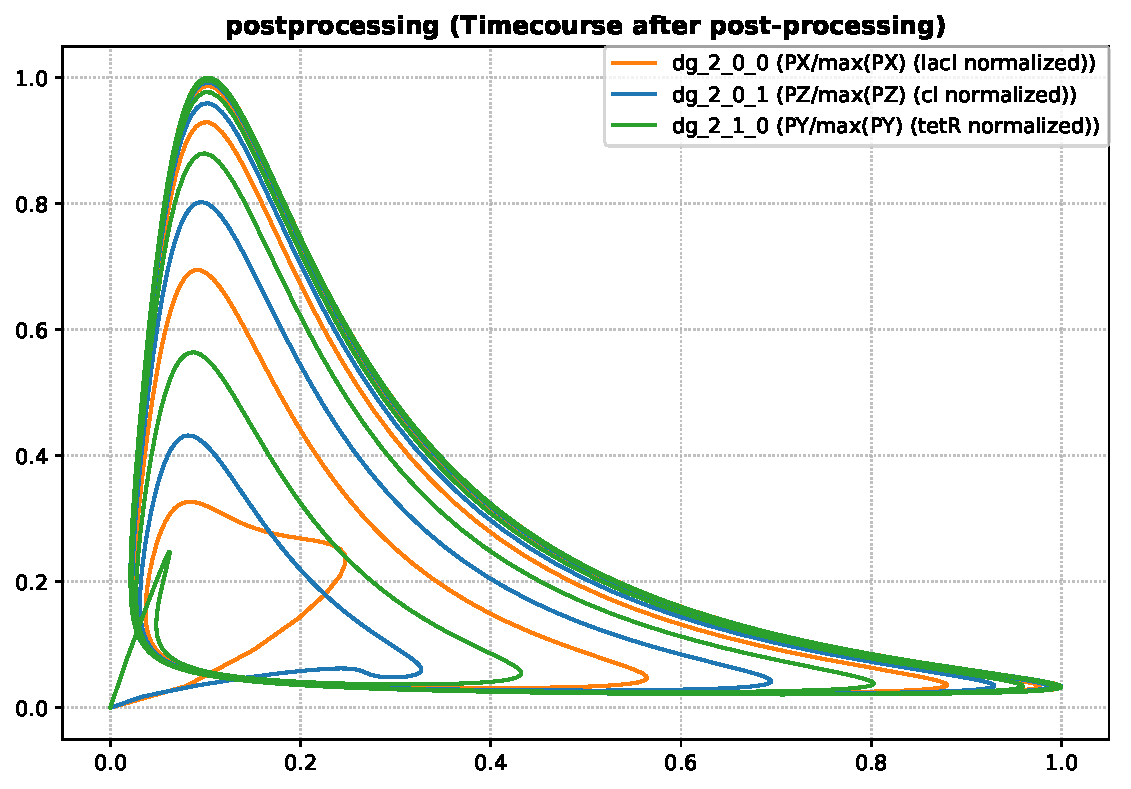
\includegraphics[width=1.0\textwidth]{examples/repressilator/results/tellurium/postprocessing}
        \caption{Time-course simulation of the repressilator. Normalized \code{lacI}, \code{tetR} and \code{cI} in phase-plane. Simulation with tellurium \citep{tellurium}.}
        \label{fig:rep_post2}
    \end{minipage}
\end{figure}
